% Modified Template by Jonathan Doucette and Kevin Multani, original by: Jonathan Ward

\documentclass[12pt]{article} 
\usepackage[english]{babel}
\usepackage[utf8]{inputenc}
\usepackage{amsmath} % AMS Math Package
\usepackage{amsthm} % Theorem Formatting
\usepackage{amssymb} % Math symbols such as \mathbb
\usepackage{graphicx} % Allows for eps images
\usepackage{multicol} % Allows for multiple columns
\usepackage[dvips,letterpaper,margin=1in,bottom=1in]{geometry}
\usepackage{hyperref}
\usepackage{parskip} % Removes indentation from paragraphs
\usepackage{xcolor,xspace,soul} % Colour, spacing, and highlighting
\usepackage{mathrsfs}
\usepackage{bm} % For bold math symbols
\usepackage{amscd}
\usepackage[all,cmtip]{xy}
%\usepackage{bbm}
\usepackage{titling}
\usepackage{listing} % for code snippets
%\usepackage{minted} % for code snippets
\usepackage{enumerate}
\usepackage{fancyhdr}
\usepackage[]{physics}
\usepackage[makeroom]{cancel}
\usepackage{pdfpages}
\usepackage[]{mcode}
\usepackage[title]{appendix}

% ***********************************************************
% ********************** BEGIN TITLE PAGE *******************
% ***********************************************************
\newcommand*{\titleGM}{\begingroup % Create the command for including the title page in the document
\hbox{ % Horizontal box
\hspace*{0.2\textwidth} % Whitespace to the left of the title page
\rule{1pt}{\textheight} % Vertical line
\hspace*{0.05\textwidth} % Whitespace between the vertical line and title page text
\parbox[b]{0.75\textwidth}{ % Paragraph box which restricts text to less than the width of the page

{\noindent\Huge\bfseries MATH 521}\\[2\baselineskip] % Title
{\large \textit{Assignment 4}}\\[4\baselineskip]
%{\large \textsc{ Jonathan Doucette }} % Author name

\vspace{0.5\textheight} % Whitespace between the title block and the publisher
{\noindent \today }\\[\baselineskip]
%{\noindent Student Number: 35298124 }\\[\baselineskip] 
%{\noindent \footnotesize All problems below are \textit{Copyright \copyright \space 2018 Timm Treskatis. All Rights Reserved.} }\\[\baselineskip]
} % end parbox
} % end hbox
\endgroup}

 % Sets margins and page size
\pagestyle{fancy} 

%\lhead{Jonathan Doucette}
\rhead{\today}
\rfoot{Page \thepage}
\cfoot{}

\makeatletter % Need for anything that contains an @ command 
\renewcommand{\maketitle} % Redefine maketitle to conserve space
{ \begingroup \vskip 10pt \begin{center} \Huge {\bf \@title}
\vskip 10pt \large \@author \hskip 20pt \@date \end{center}
  \vskip 10pt \endgroup \setcounter{footnote}{0} }
\makeatother % End of region containing @ commands

% ***********************************************************
% ********************** END TITLE PAGE *********************
% ***********************************************************

% ***********************************************************
% ********************** BEGIN NEW COMMANDS *****************
% ***********************************************************

\renewcommand{\labelenumi}{(\alph{enumi})} % Use letters for enumerate
\let\vaccent=\v % rename builtin command \v{} to \vaccent{}

%% MISC
\newcommand{\ab}[1]{\left| #1 \right|} % for absolute value
\newcommand{\avg}[1]{\left< #1 \right>} % for average
\let\underdot=\d % rename builtin command \d{} to \underdot{}
\let\baraccent=\= % rename builtin command \= to \baraccent
\renewcommand{\=}[1]{\stackrel{#1}{=}} % for putting numbers above =
\providecommand{\fr}{\frac}
\providecommand{\RR}{\mathbb{R}}
\providecommand{\CC}{\mathbb{C}}
\providecommand{\NN}{\mathbb{N}}
\providecommand{\e}{\epsilon}
\DeclareMathOperator{\di}{d\!}
\newcommand*\ieval[3]{\left.#1\right\rvert_{#2}^{#3}}

%% Vectors
\renewcommand{\v}[1]{\ensuremath{\mathbf{#1}}} 
\newcommand{\gv}[1]{\ensuremath{\mbox{\boldmath$ #1 $}}} % for vectors of Greek letters
\newcommand{\uv}[1]{\ensuremath{\mathbf{\hat{#1}}}} % for unit vector
\providecommand{\wave}[1]{\v{\tilde{#1}}}

%% DERIVATIVES
\renewcommand{\d}[2]{\frac{d #1}{d #2}} % for derivatives
\newcommand{\dubd}[2]{\frac{d^2 #1}{d #2^2}} % for double derivatives
\newcommand{\pd}[2]{\frac{\partial #1}{\partial #2}} % for partial derivatives
\newcommand{\pdd}[2]{\frac{\partial^2 #1}{\partial #2^2}} % for double partial derivatives

%% Operators
\newcommand{\Gradient}{\ensuremath{\mbox{\boldmath$\nabla$}}} % gradient

%% Text
\newcommand{\mathcolorbox}[2]{\colorbox{#1}{$\displaystyle #2$}}
\newcommand{\hlfancy}[3]{\textcolor{#1}{\sethlcolor{#2}\hl{#3}}}
\newcommand{\TODO}[1]{\hlfancy{red}{yellow}{\textbf{TODO: #1}}}

%% Code
%\newcommand{\code}[1]{\mintinline{C}{#1}}
%\newcommand{\code}[1]{\texttt{#1}}
\newcommand{\code}[1]{\lstinline[columns=fixed]{#1}}
\newcommand{\includecode}[1]{\lstinputlisting{#1}}

% ***********************************************************
% ********************** END NEW COMMANDS *******************
% ***********************************************************

% ***********************************************************
% ********************** BEGIN NEW ENVS *********************
% ***********************************************************

% Theorem
\newenvironment{theorem}[2][Theorem]{\begin{trivlist}
\item[\hskip \labelsep {\bfseries #1}\hskip \labelsep {\bfseries #2.}]}{\end{trivlist}}
% Lemma
\newenvironment{lemma}[2][Lemma]{\begin{trivlist}
\item[\hskip \labelsep {\bfseries #1}\hskip \labelsep {\bfseries #2.}]}{\end{trivlist}}
% Corollary
\newenvironment{corollary}[2][Corollary]{\begin{trivlist}
\item[\hskip \labelsep {\bfseries #1}\hskip \labelsep {\bfseries #2.}]}{\end{trivlist}}

% Exercise
\newenvironment{exercise}[2][Exercise]{\begin{trivlist}
\item[\hskip \labelsep {\bfseries #1}\hskip \labelsep {\bfseries #2.}]}{\end{trivlist}}
% Problem
\newenvironment{problem}[2][Problem]{\begin{trivlist}
\item[\hskip \labelsep {\bfseries #1}\hskip \labelsep {\bfseries #2.}]}{\end{trivlist}}
% Question
\newenvironment{question}[2][Question]{\begin{trivlist}
\item[\hskip \labelsep {\bfseries #1}\hskip \labelsep {\bfseries #2.}]}{\end{trivlist}}
% Solution
\newenvironment{solution}{\begin{proof}[Solution]}{\end{proof}}

% Afterword
\newenvironment{afterword}[2][Appendix]{\begin{trivlist}
\item[\hskip \labelsep {\bfseries #1}\hskip \labelsep {\bfseries #2}]}{\end{trivlist}}

% ***********************************************************
% ********************** END NEW ENVS ***********************
% ***********************************************************

% ***********************************************************
% ********************** END TITLEPAGE **********************
% ***********************************************************

%\documentclass[10pt,letterpaper]{scrartcl}
%\usepackage{amsfonts,amsmath,amssymb,braket,xcolor,dsfont,enumerate,fontawesome,graphicx}
\usepackage{amsfonts,amsmath,amssymb,braket,xcolor,enumerate,graphicx}
\usepackage[hidelinks]{hyperref}
\usepackage{listings,multicol,mathtools,textcomp,tikz,pgfplots,wrapfig}
%\usepackage[inner=2cm,outer=2cm,top=2cm,bottom=2cm]{geometry}
\usepackage{tabularx}
\usepackage{booktabs}
\usetikzlibrary{arrows}
%\pgfplotsset{compat=1.12}

\pagestyle{empty}
\setlength{\parindent}{0pt}
\setlength{\parskip}{6pt}

%\newcommand{\dx}{\;\mathrm{d}x}

\begin{document}

\begin{minipage}{.2\textwidth}

\includegraphics[width=42pt]{ubc-logo.png}
\end{minipage}
\hfill
\begin{minipage}{.75\textwidth}
\setlength{\parskip}{6pt}
\begin{flushright}
{\sffamily
\textbf{MATH521}\\
\textbf{Numerical Analysis of Partial Differential Equations}

Winter 2017/18, Term 2%\\
%Timm Treskatis
}
\end{flushright}
\end{minipage}

\section*{Homework Assignment 8}

Please submit the following files as indicated below:% \hfill \faFileCodeO \: source code \hfill \faFilePdfO \: PDF file \hfill \faFilePictureO \: image file \hfill \faFileMovieO \: video file

\paragraph*{If you haven't done so already, install \textsf{ParaView} on your computer.}

This is already included in many \textsf{Linux} distributions. For other operating systems, visit \url{https://www.paraview.org/download/}.

% -------------------- %
% ---- Question 1 ---- %
% -------------------- %
\paragraph*{Question 1 $\vert$ 1 mark}% $\vert$ \faFilePdfO}

This assignment is dedicated to a posteriori error estimates for the problem
\begin{equation}\tag{P}\label{eq:primal}
\begin{aligned}
-\Delta u &= f \qquad \text{in } \Omega\\
u &= 0 \qquad \text{on } \partial\Omega
\end{aligned}
\end{equation}
where $\Omega$ is the unit square $\left]0,1\right[^2$.

We want to solve this problem because we are interested in the average of $u$ over the set $R = \left]\frac{1}{2},1\right[ \times \left] 0,\frac{1}{2}\right[$.

Following the dual weighted residual method, what is the dual problem that you have to solve for $z$? Write down its weak formulation, then its strong formulation. Don't forget to specify what space the solution and the test functions belong to for the weak formulation.

\emph{Hint:} Indicator function.

% ------------------------------ %
% ---- Question 1: Solution ---- %
% ------------------------------ %
\begin{solution}
We start by rewriting the strong form \eqref{eq:primal} of the \textsc{Poisson-Dirichlet} problem into the weak form.

Since we will be solving this problem with linear finite elements (as indicated in \texttt{hw8.py}), we will take the test functions to be $v \in V = H_0^1(\Omega)$.
Additionally, since $\Omega$ is a convex polygonal domain (namely, the open unit square), we have that the space of linear finite elements $V^h \subset V$ is conforming.

As in the notes, we assume that the data $f$ is an $L^2$-function and that the exact solution is in $H^2$.
Now, multiplying \eqref{eq:primal} by $v \in V = H_0^1(\Omega)$, integrating by parts, and using that fact that $u,v = 0$ on $\partial \Omega$, the resulting weak form of the \texttt{Poisson-Dirichlet} problem is
\begin{align*}
	\int_\Omega \nabla u \cdot \nabla v \dx{x}
    = \int_\Omega f v \dx{x},
    \quad \forall \, v \in V,
\end{align*}
or
\begin{align}\tag{W}\label{eq:primal-weak}
	B(u,v) = \left\langle f, v \right\rangle,
    \quad \forall \, v \in V
\end{align}
where we have defined the bilinear form $B(u,v) \coloneqq \int_\Omega \nabla u \cdot \nabla v \dx{x}$.

Now, using the dual weighted residual method, we introduce the corresponding dual problem
\begin{align}\tag{W*}\label{eq:dual-weak}
	B(v,z) = J(v),
    \quad \forall \, v \in V
\end{align}
where $J(u)$ is the linear functional
\begin{align}\label{eq:J-defn}
	J(u) = \frac{1}{|R|}\int_R u \dx{x}
\end{align}
representing the quantity of interest, namely the average of the solution $u$ over the region $R = \left]\frac{1}{2},1\right[ \times \left] 0,\frac{1}{2}\right[$.

Now, the dual solution $z$ and test functions $v$ are both in the space $V = H_0^1(\Omega)$, and if we first note that we can write equation \eqref{eq:J-defn} as
\begin{align}\label{eq:J-indicator}
	J(u) = \int_\Omega \left\{ \frac{1}{|R|} I_R \right\} u \dx{x}
\end{align}
where
\begin{align}\label{eq:indicator}
	I_R(x) = \begin{cases}
1, \quad x \in R \\
0, \quad x \not\in R
\end{cases}
\end{align}
is the indicator function on the set $R$, then due to the symmetry $B(v,z) = B(z,v)$ of the bilinear functional $B$, the corresponding strong form of the dual problem \eqref{eq:dual-weak} is simply
\begin{equation}\tag{P*}\label{eq:dual}
\begin{aligned}
-\Delta z &= g \qquad \text{in } \Omega\\
z &= 0 \qquad \text{on } \partial\Omega
\end{aligned}
\end{equation}
where
\begin{align*}
g = \frac{1}{|R|} I_R.
\end{align*}
Note additionally that $|R| = \frac{1}{4}$ for $R = \left]\frac{1}{2},1\right[ \times \left] 0,\frac{1}{2}\right[$.

\end{solution}

\newpage

% -------------------- %
% ---- Question 2 ---- %
% -------------------- %
\paragraph*{Question 2 $\vert$ 4 marks}% $\vert$  \faFileCodeO \: \faFilePdfO}

If the source term in Problem \eqref{eq:primal} is given as
\begin{equation*}
f(x) = a(a+1)x_1^{a-1}x_2(1-x_2) +  2x_1(1-x_1^a)
\end{equation*}
for $a \geq 1$, then the analytical solution is
\begin{equation*}
\bar{u}(x) = x_1(1-x_1^a)x_2(1-x_2)
\end{equation*}
which has an average of
\begin{equation*}
\frac{3a-2+2^{1-a}}{24a+48}
\end{equation*}
over the set $R$.

For large $a$, this problem is numerically challenging: observe that $f$ becomes very large near the right boundary, while it remains comparatively small elsewhere in the domain. As a result, the solution $\bar{u}$ exhibits a sharp boundary layer near $x_1 = 1$.

%\includegraphics[width=.5\textwidth]{f.pdf}
%\includegraphics[width=.5\textwidth]{u.pdf}
%\begin{center}
%\footnotesize Source term $f$ (left) and analytical solution $\bar{u}$ (right) for $a=50$.
%\end{center}

\begin{enumerate}[(a)]
\item Download the \textsf{FEniCS} script \texttt{hw8.py} and complete the missing commands. This script should evaluate the a posteriori estimator $\eta_{L^2}\approx \lVert u^h - \bar{u} \rVert_{L^2} = \lVert e^h \rVert_{L^2}$ as derived in class (or on \textsf{Canvas}, under modules). Solve Problem \eqref{eq:primal} on the given grids to complete the following table:

\begin{center}
\begin{tabular}{cccc}
\toprule
$h$ & $\LTwoNorm{e^h}$ & $\eta_{L^2}$ & $\eta_{L^2} / \LTwoNorm{e^h}$\\
\toprule
$\frac{1}{64}\sqrt{2}$  & 0.00241963657483  & 0.066093085134   & 27.3152942973 \\
($64\times 64$ grid) \\
\midrule
$\frac{1}{128}\sqrt{2}$ & 0.000648344109077 & 0.0170555074095  & 26.3062580052 \\
($128\times 128$ grid)\\
\midrule
$\frac{1}{256}\sqrt{2}$ & 0.000162164095122 & 0.00437467584739 & 26.9768461638 \\
($256\times 256$ grid)\\
\bottomrule
\end{tabular}
\end{center}
Is the error overestimated or underestimated by $\eta_{L^2}$? By what factor, approximately?

\begin{solution}

The global $L^2$-norm error of the solution is overestimated by approximately a factor of 27 by $\eta_{L^2}$.

\end{solution}

\vspace{3em}

\item Compute a posteriori estimators $\eta_{J}\approx \lvert J(u^h) - J(\bar{u}) \rvert = \lvert J(e^h) \rvert$ for the error in the average solution value on $R$, using both the expensive Strategy 1 and the cheap Strategy 2 to approximate the dual weights (cf p 55 in the notes). Complete the following table:

\begin{center}
\begin{tabular}{cccccc}
\toprule
$h$ & $\lvert J(e^h) \rvert$ & $\lvert \eta_{J,1} \rvert$ & $\lvert \eta_{J,2} \rvert$ & $\lvert \eta_{J,1} / J(e^h) \rvert$ & $\lvert \eta_{J,2} / J(e^h) \rvert$\\
\toprule
$\frac{1}{64}\sqrt{2}$  & 0.000566634238416 & 0.000778386852158 & 0.000713320888805 & 1.37370246869 & 1.25887360919\\
($64\times 64$ grid)\\
\midrule
$\frac{1}{128}\sqrt{2}$ & 0.000157153783317 & 0.000187641158623 & 0.000170875597462 & 1.19399708147 & 1.08731456447\\
($128\times 128$ grid)\\
\midrule
$\frac{1}{256}\sqrt{2}$ & 3.98056031191e-05 & 4.55743743355e-05 & 4.13531013218e-05 & 1.14492359779 & 1.0388763913\\
($256\times 256$ grid)\\
\bottomrule
\end{tabular}
\end{center}
Is the error overestimated or underestimated? By what factor, approximately?

\begin{solution}

The error appears to be overestimated by a factor which is on the order of 1 and decreasing with $h$, possibly to a number below 1 but it is hard to tell, and my laptop runs out of memory when further refining the grid.

\end{solution}

\vfill

\item% \faFilePictureO \:
For the convergence studies above we have refined the entire mesh from $64 \times 64$ to $128 \times 128$ to $256 \times 256$. The second mesh is four times larger, the third mesh even 16 times larger than the coarsest one. This makes uniform mesh refinement very expensive. We can probably compute a solution that is just as accurate as the solution on the $256 \times 256$ mesh, by refining only those triangles on the $64 \times 64$ mesh with a noteworthy contribution to the overall error.

Solve Problem \eqref{eq:primal} on the $64 \times 64$ mesh and plot the numerical solutions $u^h$ and $z^h$, the cell residuals $\lVert r_T \rVert_{L^2}$, the dual weights $\lVert w_T \rVert_{L^2}$ (approximated with either the expensive or the cheap strategy) and the local error indicators $\eta_T$. What triangles of the $64 \times 64$ mesh would you refine to compute the average of $u$ over $R$ more accurately? A rough description like `near the left boundary' will do. Also give a brief reason for your answer:

\begin{solution}

Inspecting the cell residuals and the dual weights (figures \ref{fig:rT} and \ref{fig:wT} in Appendix \ref{SolnFigures}), we see that error in the average of $u$ over $R$ comes primarily from two sources: first, error occurs due to the boundary layer near $x=1$ as seen by $\LTwoNorm{r_T}$; second, $\LTwoNorm{w_T}$ shows that error occurs along the discontinuity of the indicator function, i.e. inside the domain at the boundary between $R$ and the rest of $\Omega$.

When compararing the relative effect of these two sources of error we can use the local error indicators $\eta_T$ which take both $r_T$ and $w_T$ into account.
From the plot of $\eta_T$ (Figure \ref{fig:nT}), we see that the error along the boundary layer dominates, and so the cells near the edge $x=1$ should be refined in order to most effectively lower the error of the function $J(u)$ with the least computational effort.

\end{solution}

\vfill
\end{enumerate}

\paragraph*{(Optional) Bonus Question $\vert$ 1 bonus mark}% $\vert$ \faFilePdfO}

Derive an \textit{a priori} estimate for the error in the above quantity of interest. Does it agree with the numerical results from Q2(b)?

\begin{solution}

From \textsc{Theorem 2.3.22 (Convergence in the $L^2$-Norm)} in the notes, we have that, for linear finite elements, the error $e^h = \bar{u} - u^h$ of the \textsc{Poisson-Dirichlet} problem satisfies
$$ \LTwoNorm{e^h} \leq c h^2 \ANorm{f}{L^2(\Omega)} $$
for some positive constant $c$.

Now, since the quantity of interest $J(u)$ is linear with respect to $u$, we have that $J(\bar{u}) - J(u^h) = J(\bar{u} - u^h) = J(e^h)$, and so
\begin{align*}
\abs{ J(e^h) } &= \abs{ \int_\Omega \left\{ \frac{1}{|R|} I_R \right\} e^h \dx{x} } \\
&\leq \frac{1}{|R|} \LTwoNorm{I_R} \LTwoNorm{e^h} \\
&\leq 2 c h^2 \ANorm{f}{L^2(\Omega)}
\end{align*}
where we have applied Cauchy-Schwarz in line two, and used $|R| = 1/4$, $\LTwoNorm{I_R} = 1/2$ in line 3, as well as the theorem quoted above.

Therefore, from this estimate we expect that $|J(e^h)|$ should decrease proportional to $h^2$. Inspecting the numerical results from Q2(b), we see that upon refining the grid size by factors of 2, $|J(e^h)|$ decreases by factors of approximately 3.6056 and 3.9480 with decreasing $h$, approaching the theoretical rate of $2^2=4$. Therefore, yes, the \textit{a priori} error estimate does indeed agree with the numerical results.

\end{solution}

\vfill
\newpage

\paragraph*{Your Learning Progress}% $\vert$ \faFilePdfO}

What is the one most important thing that you have learnt from this assignment?

\vspace*{3mm}

\begin{itemize}
\item More \textsf{FEniCS}! It is a fun library to use, and clearly you can easily do lots of interesting things with it.
\end{itemize}

\vspace*{5mm}

Any new discoveries or achievements towards the objectives of your course project?

\vspace*{3mm}

\begin{itemize}
\item I think the dual weighted residual method will be extremely useful for me - just need to learn how to apply it in the context of parabolic PDEs.
\end{itemize}

\vspace*{5mm}

What is the most substantial new insight that you have gained from this course this week? Any \emph{aha moment}?

\vspace*{3mm}

\begin{itemize}
\item No particular \emph{aha moment}, but this was a pretty intuitive experiment, so I'm glad to see it line up with intuition.
\end{itemize}

\vspace*{3mm}


\newpage
\begin{appendices}
\lhead{}

\section{}\label{SolnFigures}

{\centering
\null\vfill
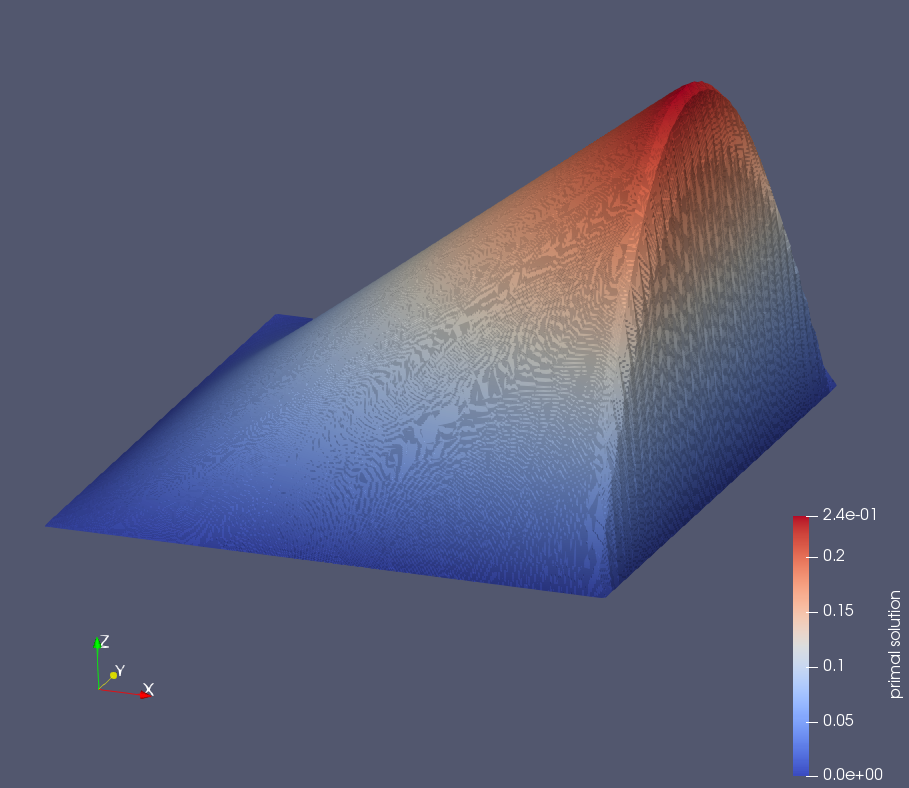
\includegraphics[width=6in, height=4in]{../fenics/images/uh.png}
\captionof{figure}{Solution $u^h$\label{fig:uh}}
\vfill
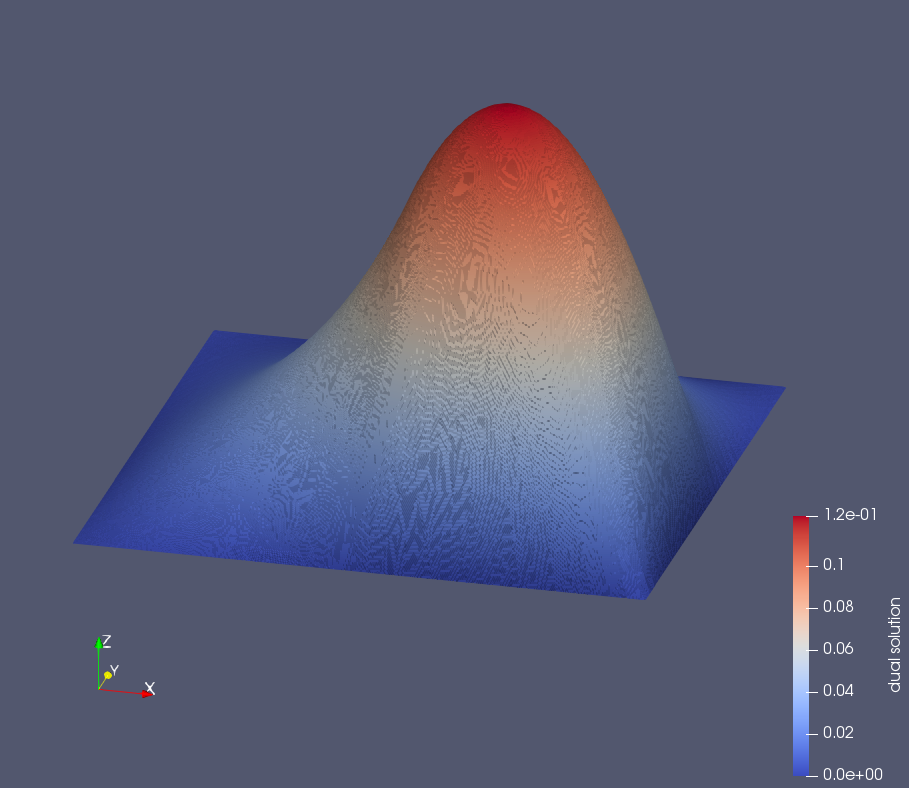
\includegraphics[width=6in, height=4in]{../fenics/images/zh.png}
\captionof{figure}{Dual solution $z^h$\label{fig:zh}}
\vfill
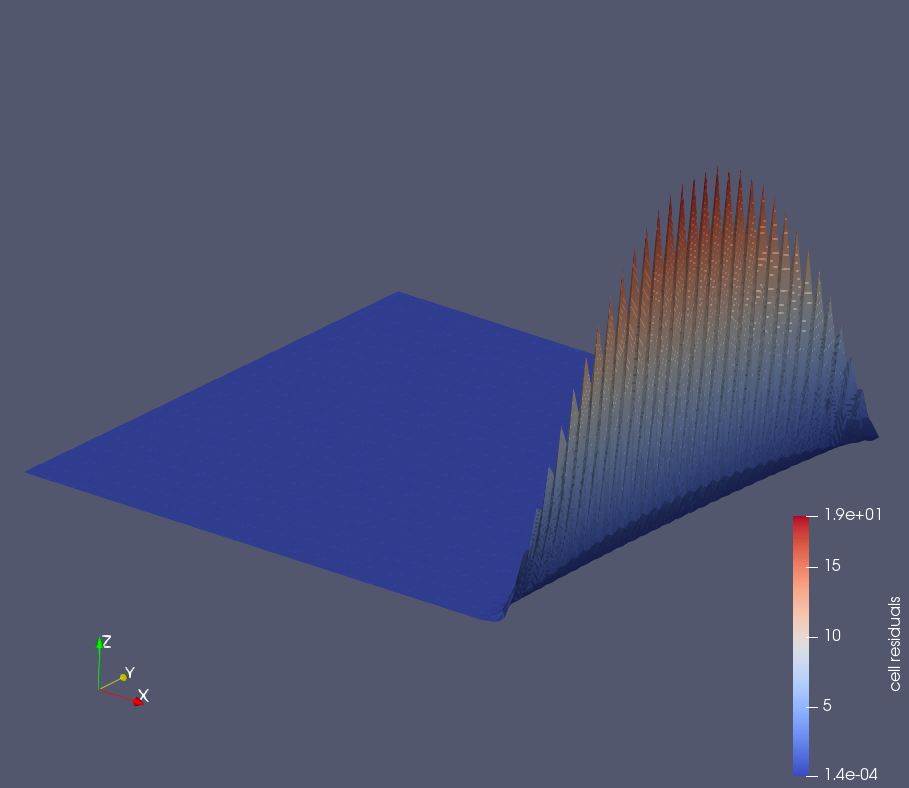
\includegraphics[width=6in, height=4in]{../fenics/images/rT.png}
\captionof{figure}{Norm of cell residuals $\LTwoNorm{r_T}$\label{fig:rT}}
\vfill
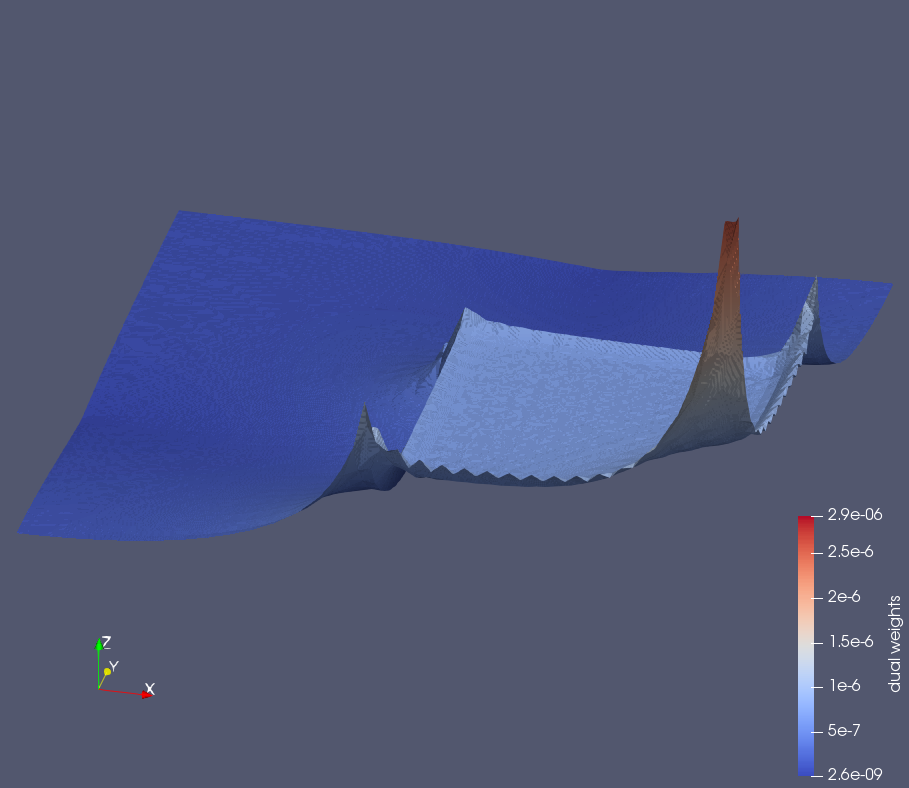
\includegraphics[width=6in, height=4in]{../fenics/images/wT.png}
\captionof{figure}{Norm of dual weights $\LTwoNorm{w_T}$\label{fig:wT}}
\vfill
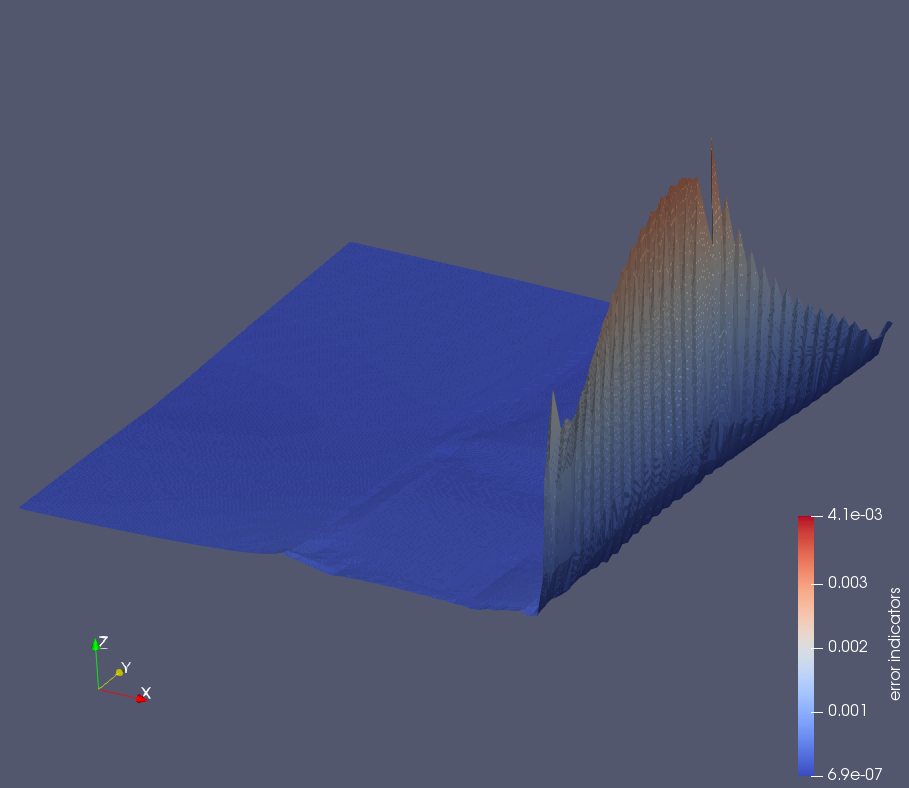
\includegraphics[width=6in, height=4in]{../fenics/images/nT.png}
\captionof{figure}{Local error indicators $\eta_T$\label{fig:nT}}
\vfill\null
}

\pagebreak

\section{}\label{hw8Code}
\textbf{\code{hw8.py}}

\hlfancy{red}{yellow}{\textbf{NOTE: UNICODE IS NOT DISPLAYED CORRECTLY. SEE THE ATTACHED FILE.}}
\includecode{../fenics/hw8.py}

\end{appendices}

\end{document}
